% !TeX spellcheck = en_GB
%======================================================================
%===  dtuposter - a class to make posters tha comply with the DTU CI
%
% Written and maintained in 2011-2014 
% by Jorrit Wronski (jowr@mek.dtu.dk)
%
%
%==========================================
%===  details and poster setup
\documentclass[
    ,title     = {{Image Segmentation for Smart Agriculture}}
%    author    = {{Soeren Winkel Holm}}
    ,subject   = {{This is the subject of my work}}
%    ,bgcolor   = dtulightgreen
%    ,highlight = dtuyellow
%    ,toplogo   = {{tex_dtu_aqua_b_uk}}
%    ,botlogo   = {{tex_dtu_bibliotek_b_uk}}
    ,papersize = {{a1paper}}
%    ,colcount  = {{1column}}
%    ,longtitle
%    ,largecaption
%    ,final
    ,nocrop
%    ,english        % language
%    ,fleqn          % equations on the left
]{dtuposter}
%
%
%======================================================================
%===  Continue with packages
\usepackage[T1]{fontenc}        % special characters

\usepackage[nottoc, numbib]{tocbibind}
%\usepackage[ansinew]{inputenc}  % Windows
%\usepackage[applemac]{inputenc} % MacOS
\usepackage[utf8]{inputenc}    % Unicode, Linux

%
% 
%======================================================================
%=== Font definitions, DTU recommends Arial for posters
%\usepackage{cmbright}
%\usepackage{arevmath}
%\usepackage[scaled]{uarial} %Arial clone, set as default sf font - use "ua1" for direct access
%\usepackage{uarial} %Arial clone, set as default sf font - use "ua1" for direct access
%\usepackage[typeface=default,
%            sanstypeface=urwarial,
%            mathtypeface=arevmath
%           ]{typeface}
\renewcommand{\familydefault}{\sfdefault}
\usepackage{enumitem}
\usepackage{mathtools}
\setlist{nosep,leftmargin=*}
%
% 
%======================================================================
%=== Other useful packages
\usepackage{booktabs}

\usepackage{float}
\usepackage[caption = false]{subfig}
%======================================================================
%=== The actual content starts here
\begin{document}
%
%
%======================================================================
%===  Make header for poster (title and authors)
\begin{dtuposterhead} %
\dtuposterauthor{\normalsize Mads Andersen, Oskar Wiese, Anders Henriksen, Søren Holm, Asger Schultz}
\dtuposteraffil{\small DTU Compute}
\dtuposteraffil{\small \texttt{\{s173934, s183917, s183904, s183911, s183912\}@student.dtu.dk}}
\end{dtuposterhead}
%
%
%======================================================================
%===  ... and the rest of the content
\begin{dtupostercontent}
\section{The Story to be Told}
\begin{itemize}
	\item Agriculture can be made more efficient by using automization to seperate the crops from the weeds and the dirt.
	\item On this poster, you can expect to learn about the implementation of SegNet for pixelwise crop classification on a drone image. The results of this implementation is also shown as well as how they came to be.
\end{itemize}
 
\section{The Data: Brazilian Sugar Fields}
The data used in this project is one drone image of a field, which is illustrated as the following.
\begin{figure}
\centering
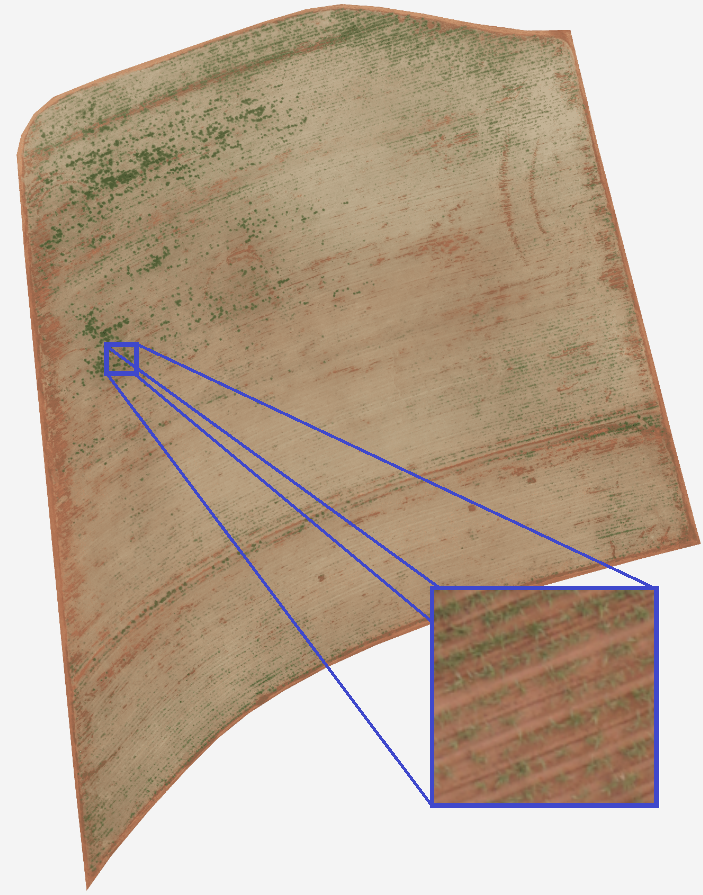
\includegraphics[width=.7\linewidth]{raw-min3}
\caption{Orthomosaic drone photo of a sugar cane field in Brazil.}
\end{figure}
\begin{itemize}
	\item Labelling of the field is performed by biologist into 3 categories: crops, weeds and soil.
	\item The goal of our project is to train a neural network that can perform a pixelwise classification on a field.
	\item Augmentation techniques has been used to expand our data set.
\end{itemize}

\section{Our SegNet: 1152 Feature Maps}


%%Model af netværket 
%%Encoder-Decoder
%% "Skip connections"" + Adam 

\begin{figure}
	\centering
	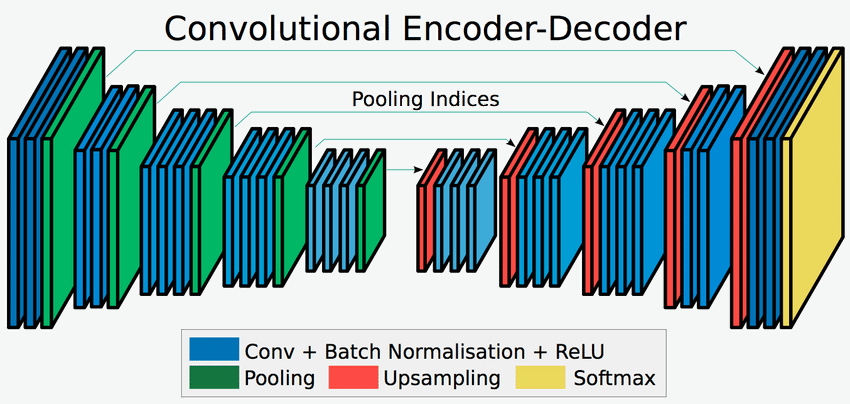
\includegraphics[width=0.9\linewidth]{Encoder-Decoder2}
	\caption{The structure of the network. Dropout prevents overfitting, batchnorm normalizes, ReLU creates non-linearity and max-pool helps with translational invariance.}
	\caption{}
	\label{fig:Structure}
\end{figure}

\begin{itemize}
	\item Same but mirrored encoder and decoder dimensions means ample opportunity for pixel-wise classification!
\end{itemize}
 
%\begin{figure}
%	\centering
%	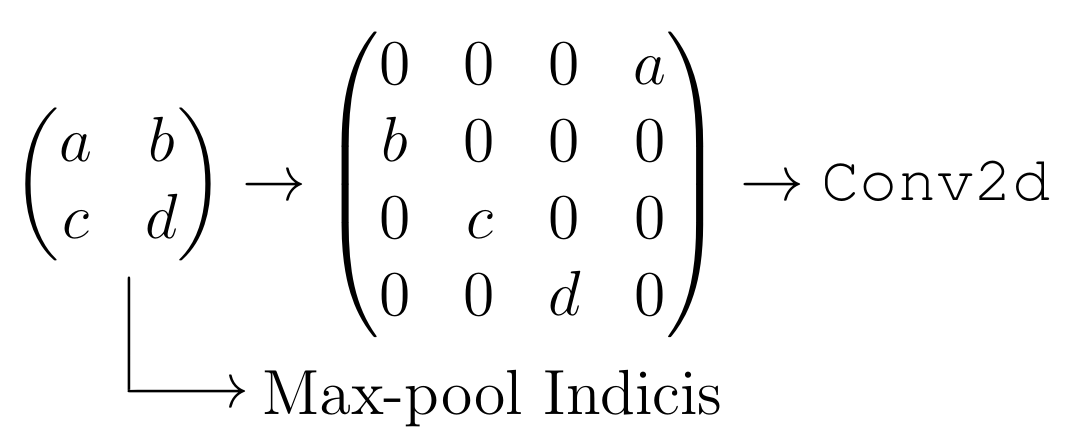
\includegraphics[width=1\linewidth]{pool}
%	\label{fig:maxpool}
%\end{figure}
\subsubsection*{Skip Connections}
The skip connections used in SegNet are the max-pooling indices from the encoder-layer. These indices are used for the up-sampling in the decoder-layers. The process is illustrated as the following:
\begin{equation*}\label{key}
\scriptsize
\begin{bmatrix}a&b\\c&d\end{bmatrix} \xrightarrow{\text{\scriptsize M. pool indices}}
\begin{bmatrix}0&0&0&a\\b&0&0&0\\0&c&0&0\\0&0&d&0\end{bmatrix} 
\rightarrow 
\texttt{\scriptsize Conv2d}
\end{equation*}

Loss of \(N\) pixels in one-hot \((N \times  3)\) matrix \(\mathbf x^\text{pred}\) with the true classes \(\mathbf c\).
\[
L = \underbrace{
\vphantom{\sum_{i}}
\frac 1 N}
_{\mathllap{\text{Mean over minibatch}}}
\sum_{\mathclap {i=1}}^{N}
\underbrace{ 
\vphantom{\sum_{i}}
\mathbf{w}[i, c_i]}
_{\mathclap{\text{Class weight}}}  
\cdot 
\underbrace{
\log 
\frac
{-\exp\mathbf x^\text{pred}[i, c_i]}
{\sum_{j=1}^{3}\exp\mathbf x^\text{pred}[i, j]}
}_{\mathclap{\text{3-class cross entropy}}}
\]
\begin{figure}
	\begin{center}
			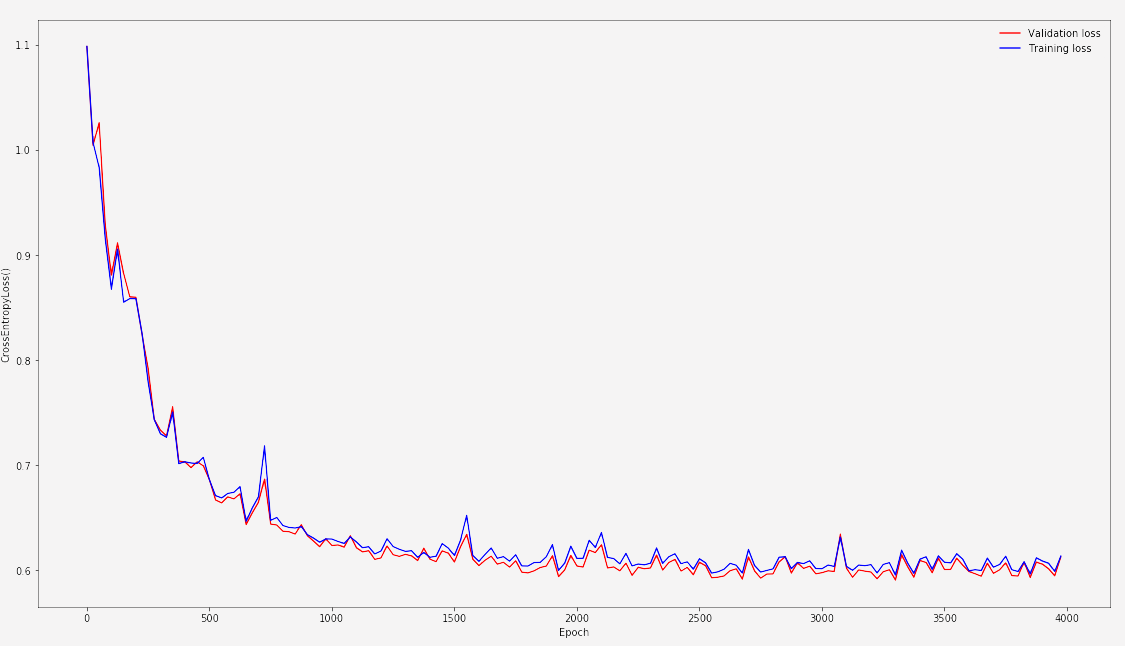
\includegraphics[width=\linewidth,origin=c]{loss2}
	\end{center}
	\caption{A plot of the training and evaluation loss as a function of the number of epochs. The validation loss is red and the training loss is blue.}\label{fig:example2}
\end{figure}

%% Hvordan regulariseres netværket
%% Data transformeringer 
%% Hyperparametre 
\section{Reconstruction}
\begin{figure}
	\centering
	\includegraphics[width=0.7\linewidth]{"Reconstruction DL"}
	\caption{Due to worse quality of border predictions, we have padded the smaller images to increase performance near borders.}
	\label{fig:reconstruction-dl}
\end{figure}
\begin{itemize}
	\item Inference is performed on smaller images, for practical reasons.
	\item Quality of predictions near borders are bad, our solution is to add padding and cut away border predictions.
	\item This results in a smooth unified field prediction, when the smaller images are stitched .
\end{itemize}


\section{Different Metrics, Different Stories}


%%Tabel med metrics 
%% Gøre vores F1 score fed og skriftstørrelse 100
\begin{table}
	\centering 
	\begin{tabular}{l|cccc|cccc}
		
		\rule[-1ex]{0pt}{2.5ex}  & \multicolumn{4}{c|}{Train} &  \multicolumn{4}{c|}{Test} \\ 
		
		\rule[-1ex]{0pt}{2.5ex} Metric  & G & C &mIoU&  mF1 & G & C & mIoU& mF1 \\ 
		\hline
		\rule[-1ex]{0pt}{2.5ex} Baseline& 91& 33 &30  &32  &94  &33  &31 &32  \\ 
		
		\rule[-1ex]{0pt}{2.5ex} USC. SegNet    &  &  &  &  &  & &   80 &96  \\ 
		\rule[-1ex]{0pt}{2.5ex} USC. UNet   &  &  &  &  &  & &75 &93  \\ 
		\rule[-1ex]{0pt}{2.5ex} Cellari DNN   &  &  &  &  &  & & &78  \\ 
		\hline 
		\rule[-1ex]{0pt}{2.5ex} Our SegNet & 97 & 87 & 80 &88  & 98  &80&74&\textbf{84}  \\ 
	\end{tabular} 
\caption{Results for different accuracy measures explained below. USC is the first work on the data set \cite{USC.} Note that we don't have access for full results for other implementations and, importantly, that the USC. implementations do not have the same train/test-split as ours.}
\end{table}

\begin{itemize}
	\item \textit{Global accuracy (G):} Simple accuracy over all pixels. Good for smooth prediction but easy to achieve optimize on unbalanced data.
	\item \textit{Mean class wise accuracy (C):} Naïve mean over class accuracies. What is being optimized for with the loss function.
	\item \textit{Mean intersect over union (mIoU):} Higher correlated to human classification. Favours regional smoothness over boundary accuracy.
	\item \textit{Mean F1 score: (mF1)} The benchmark: Penalizes false positives and gives less credit to true negatives and is thus better for unbalanced classes. 
\end{itemize}


%Kort beskrivelse af resultater 

\begin{figure}
	\centering
\subfloat{
	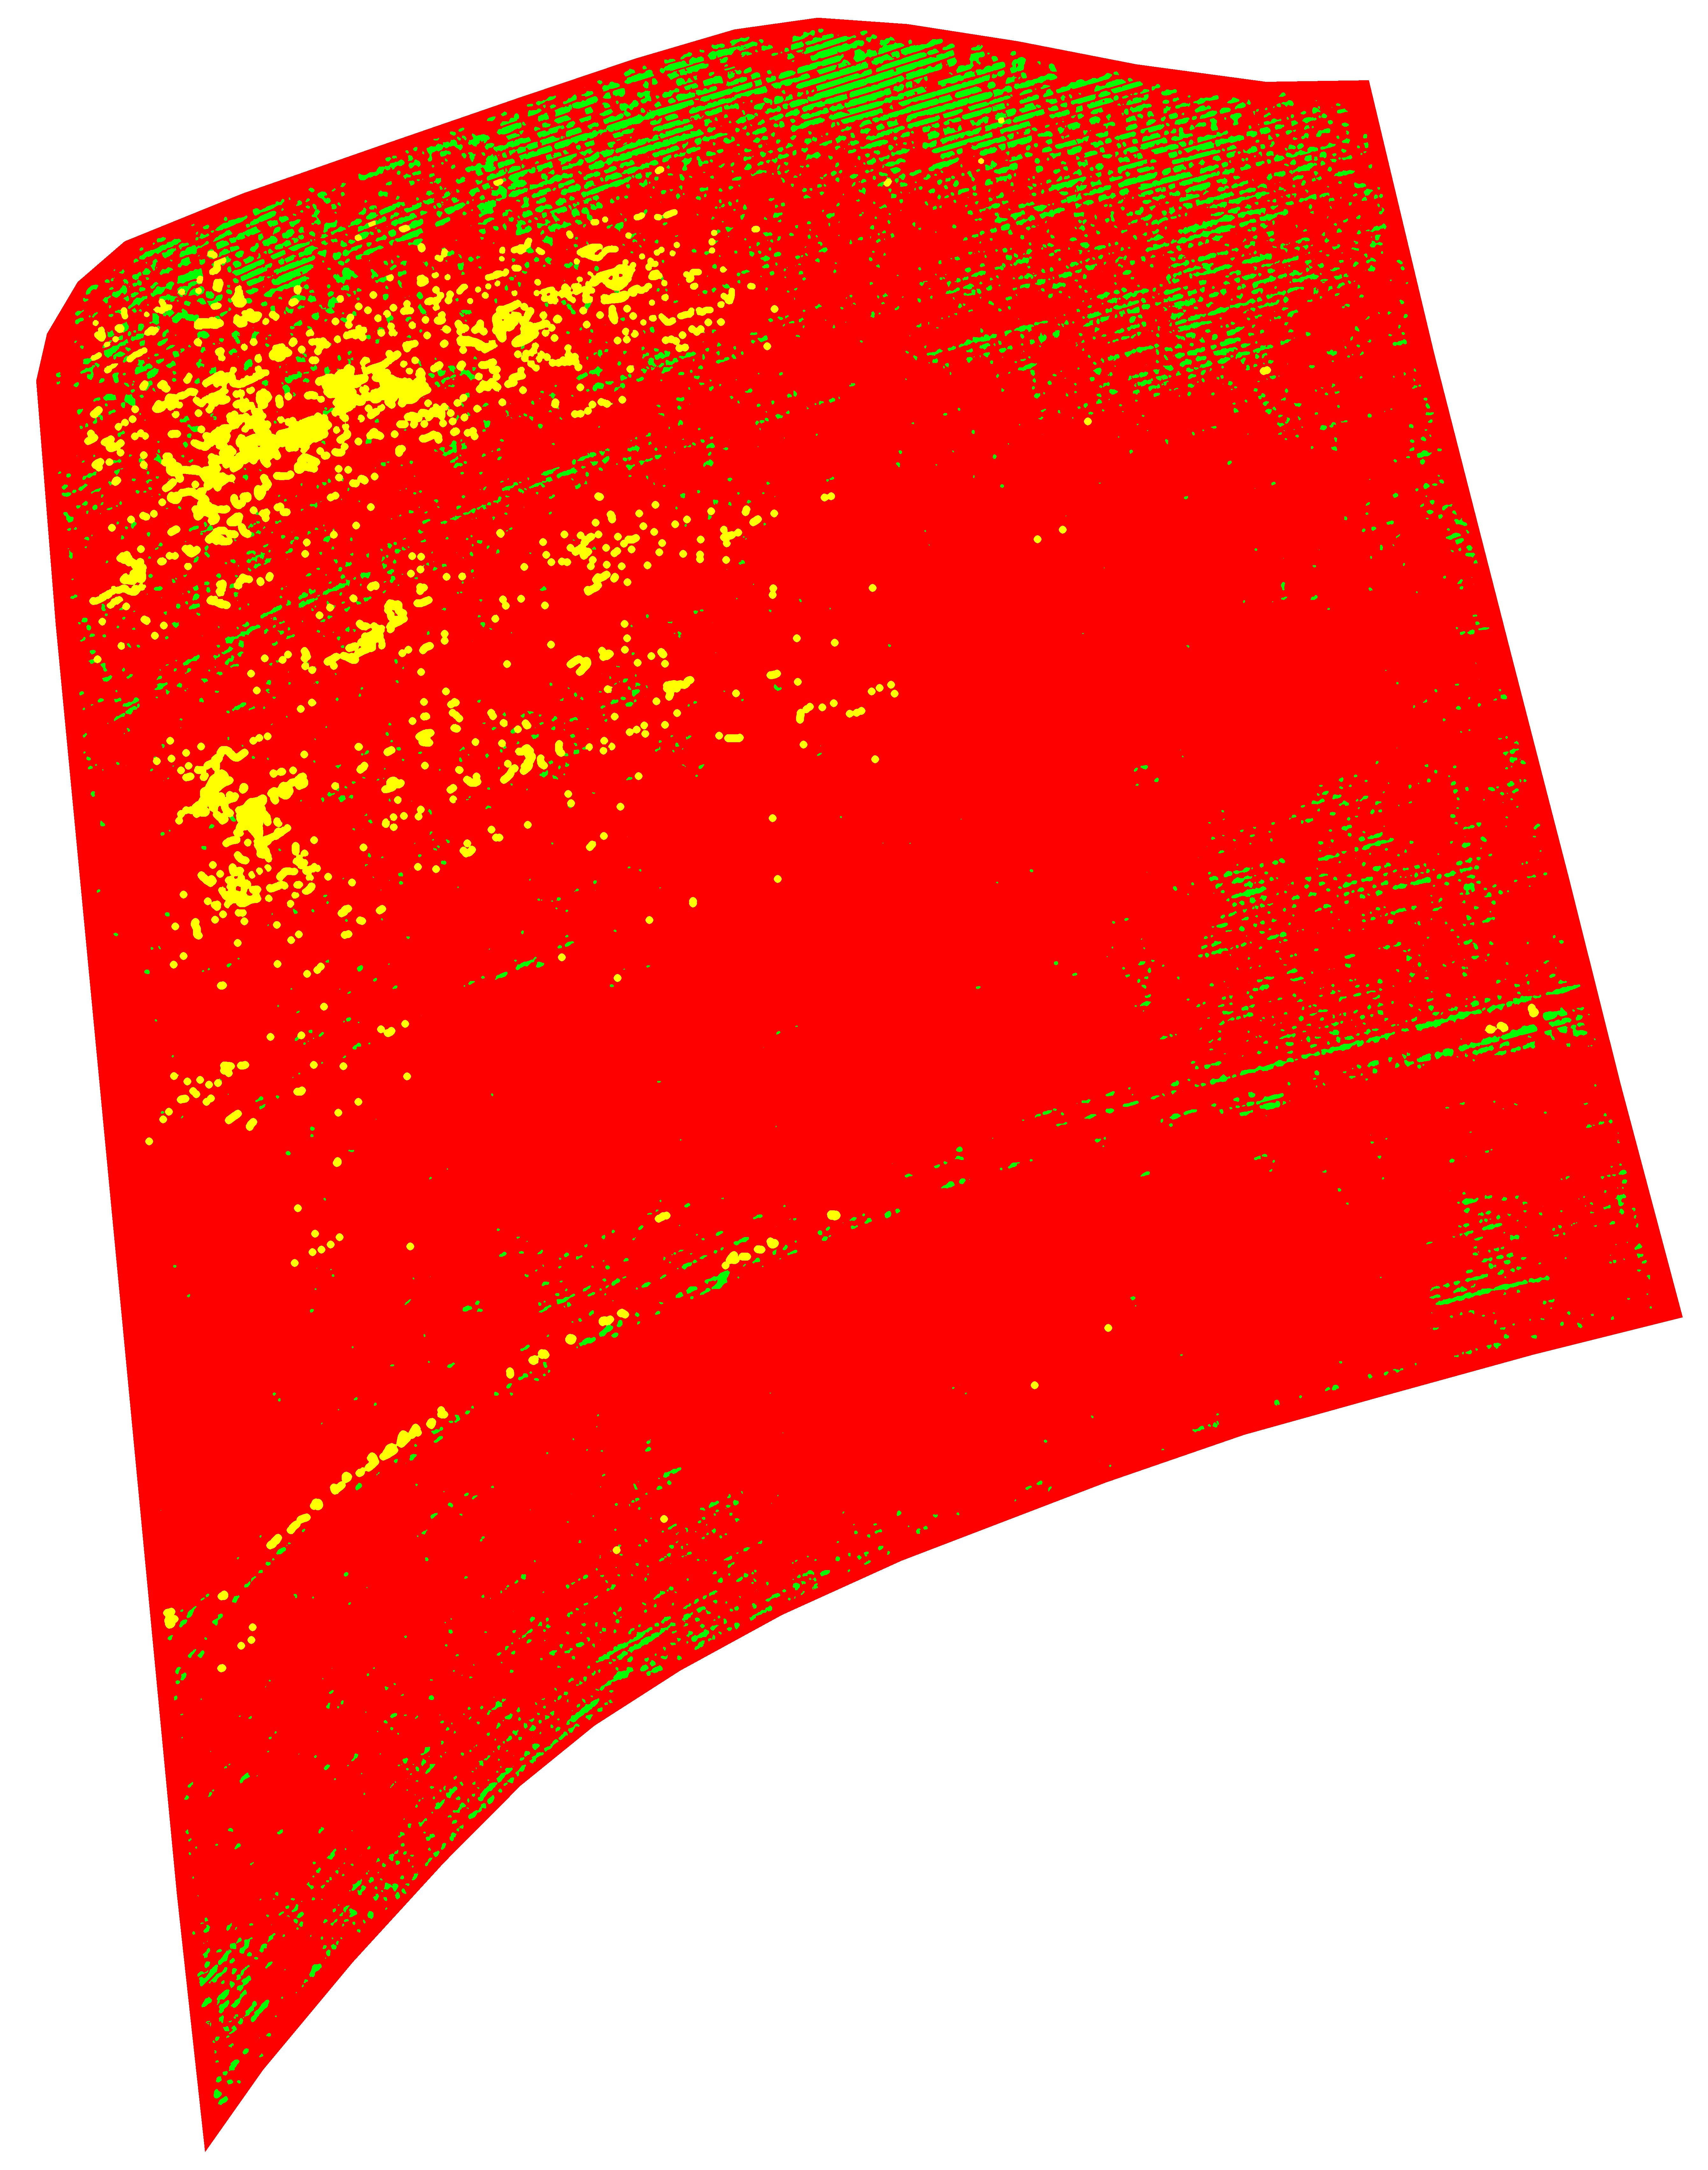
\includegraphics[width=.5\linewidth]{target2}	
}
\subfloat{
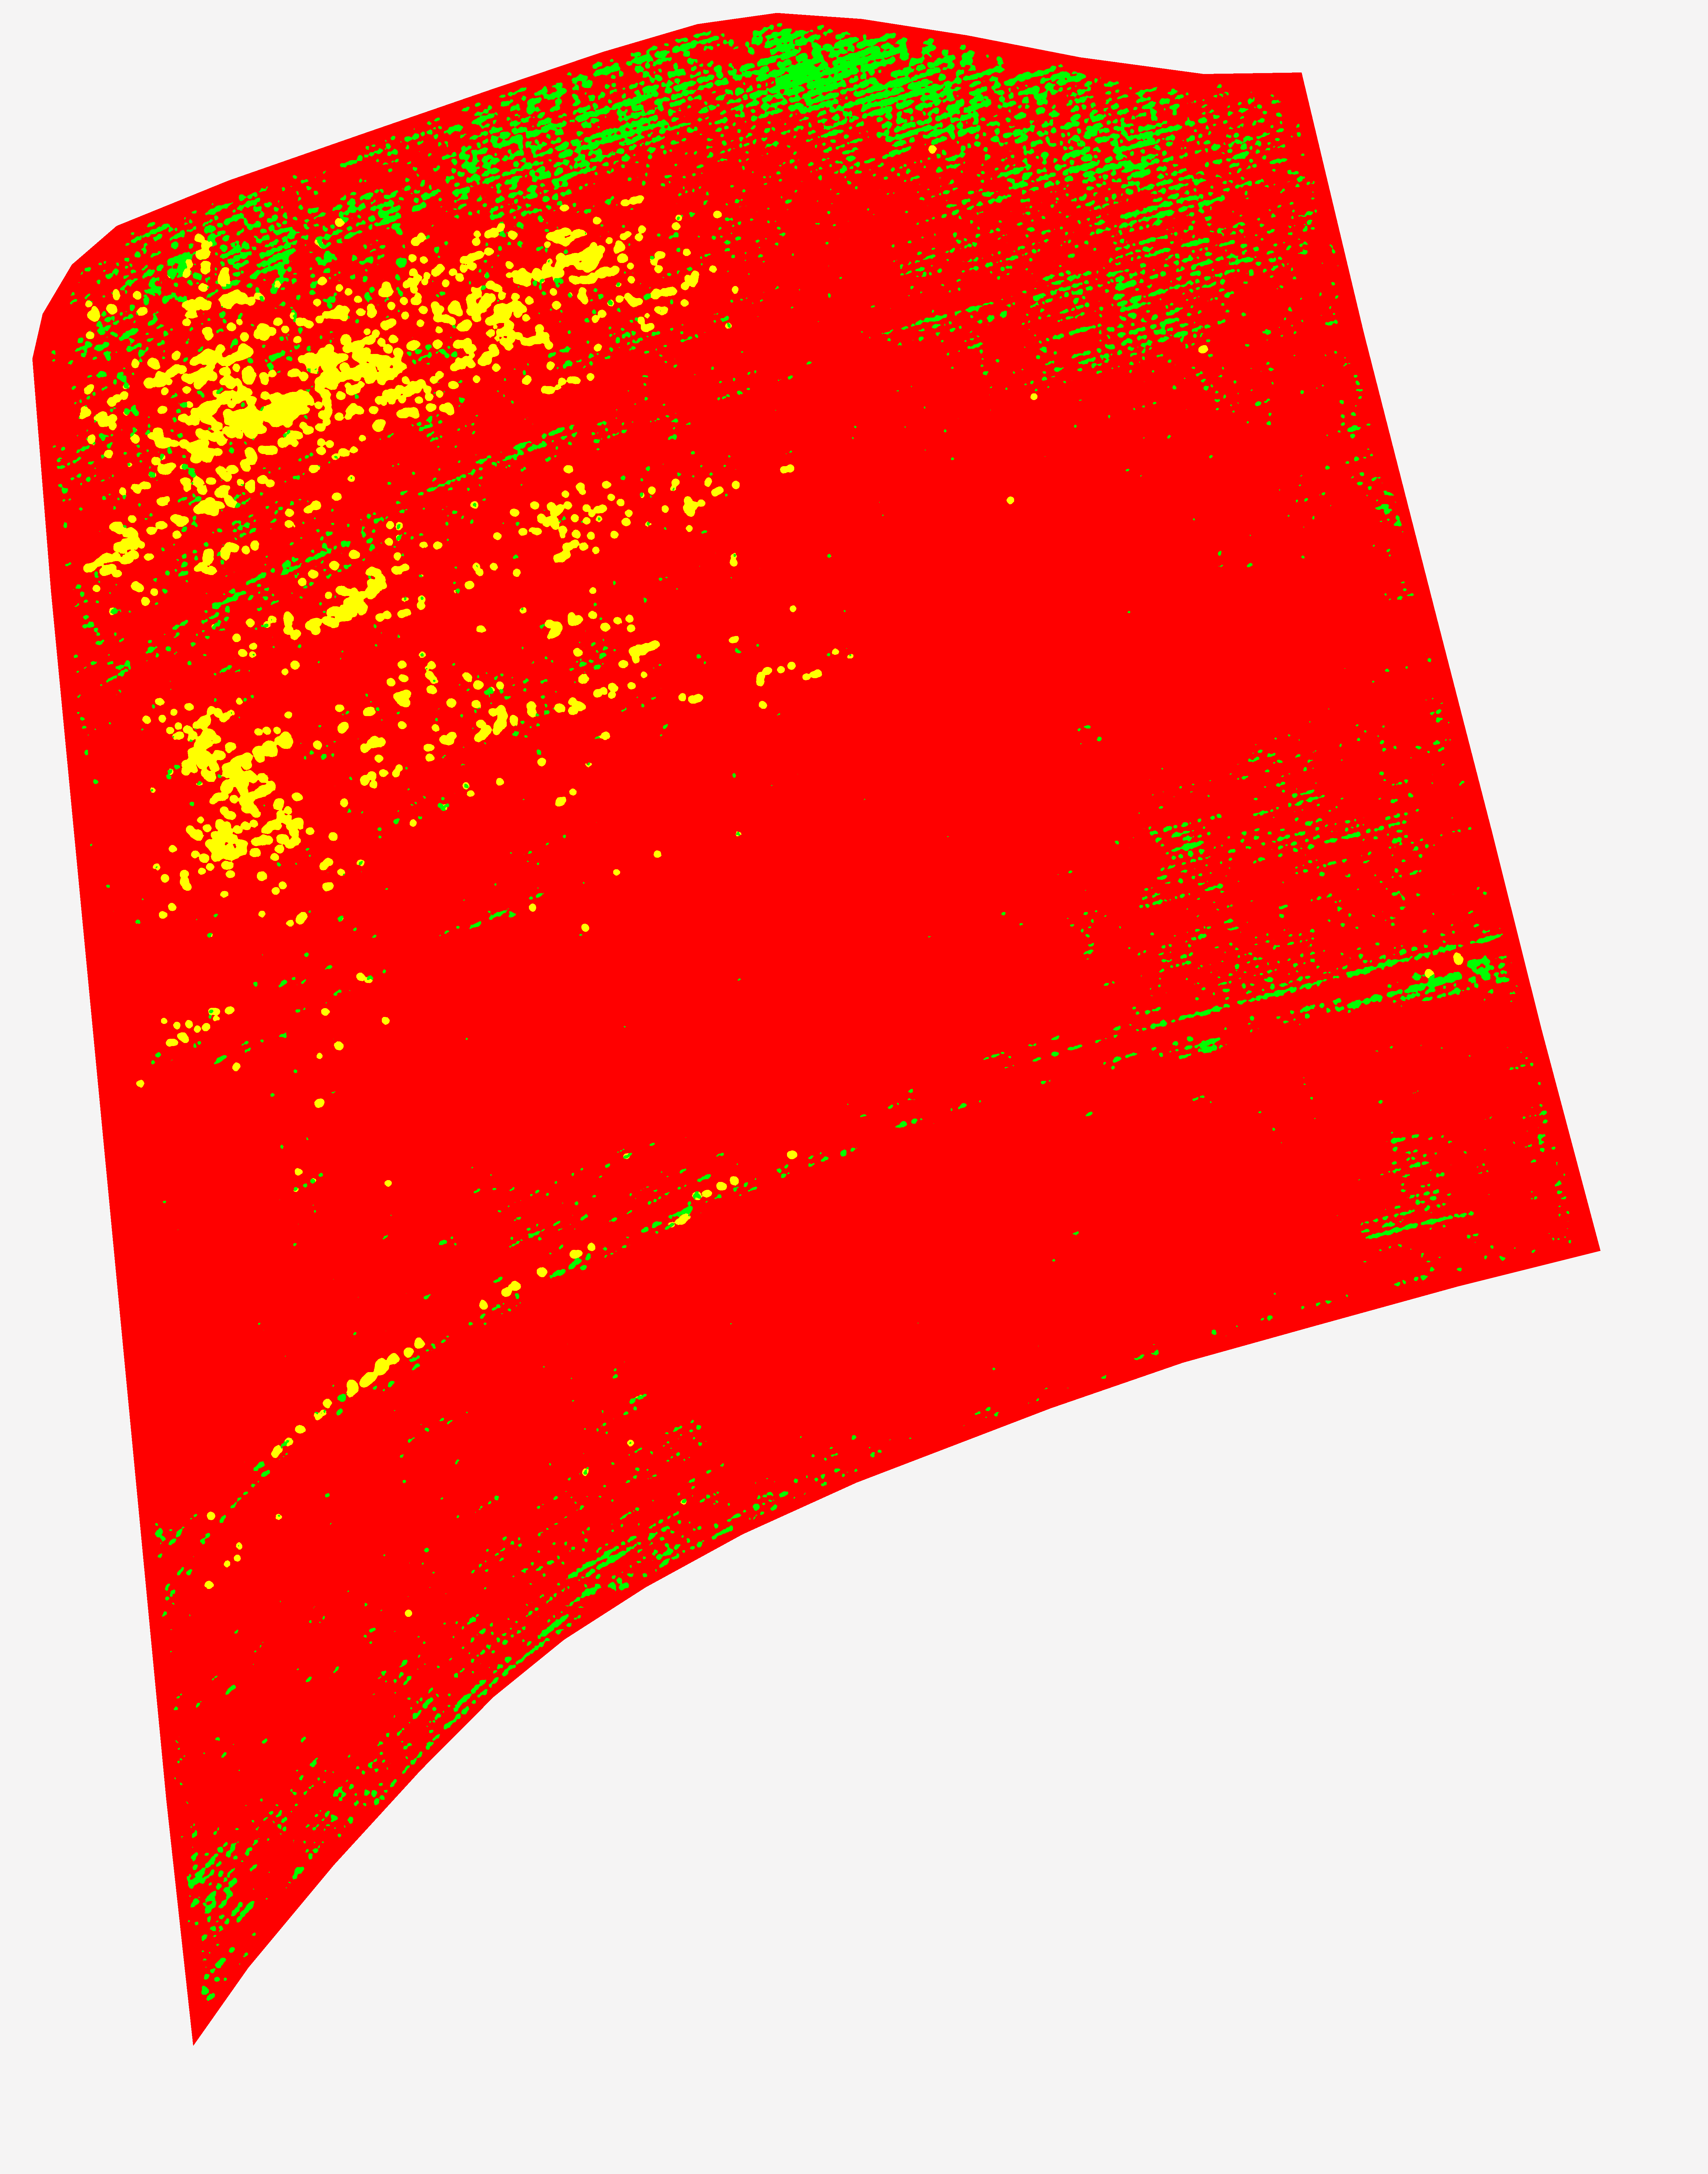
\includegraphics[width=.5\linewidth]{anno}	
}
\caption{This figure illustrates the target GT(left) as well as the predictions of the trained network(right).}\label{fig:example}
\end{figure}



\section{Where Can This Go?}
% Yderligere arbejde
%Perspektiv på problemet 

\begin{figure}
	\begin{center}
			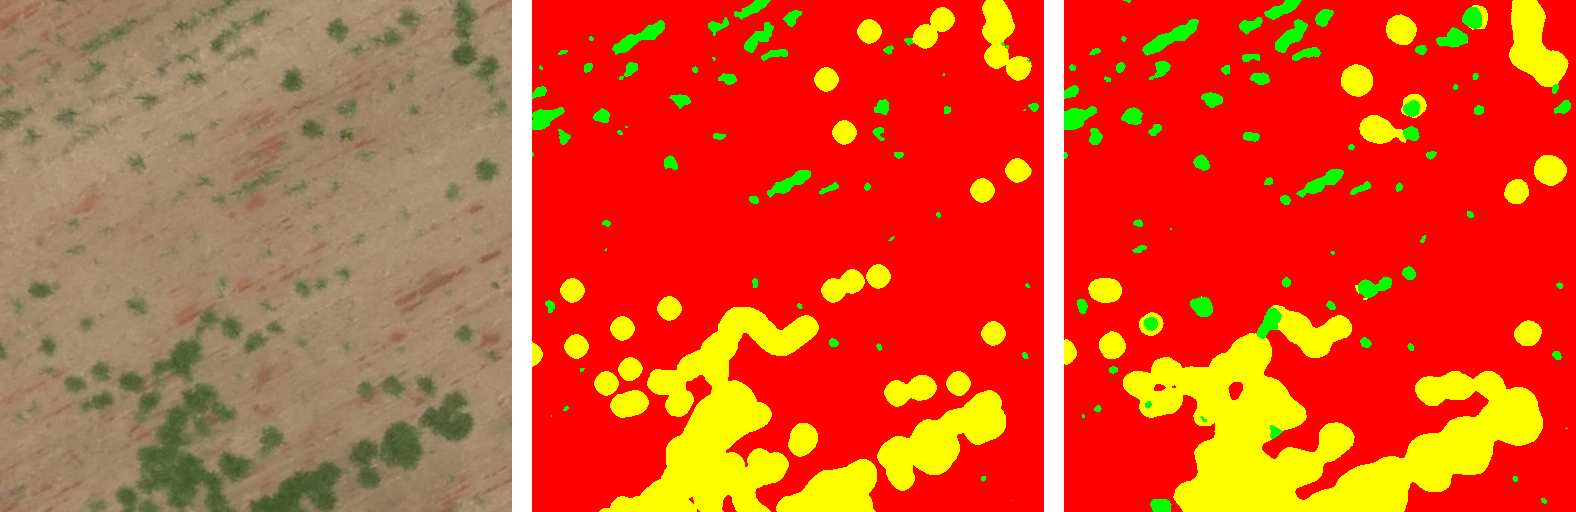
\includegraphics[width=\linewidth,origin=c]{reconst}
	\end{center}
\end{figure}

\begin{itemize}
	\item Complications with the task of image segmentation is the limited amount of data available. 
	\item More data and more advanced data augmentation can lead to a more generalizable and robust model.
	\item Can lead to an algorithm that can indentify crops and weed on a field and aid farmers in their work. 
\end{itemize}

\begin{thebibliography}{9}
	\bibitem{Seg} Kendall, Alex et al.: "SegNet: A Deep Convolutional Encoder-Decoder Architecture for Image Segmentation". PAMI, 2017.
	\bibitem{USC} Wangenheim von, Aldo et al.: "Weed Mapping on Aerial Images". INCoD.LAPIX.01.2019.E.
\end{thebibliography}
\end{dtupostercontent}


\end{document}
